\setlength{\columnsep}{3pt}
\begin{flushleft}

\bigskip
\begin{itemize}
	\item Problem with password based SSH is, you need to \textbf{share remote user's account password} in order to take its access.
	\item This can be a security problem.
	\item \textbf{Solution: Passwordless or Key based SSH}.
	\item Passwordless SSH uses a public \& private key-pair instead of user's account password while taking remote access.
	\begin{figure}[h!]
		\centering
		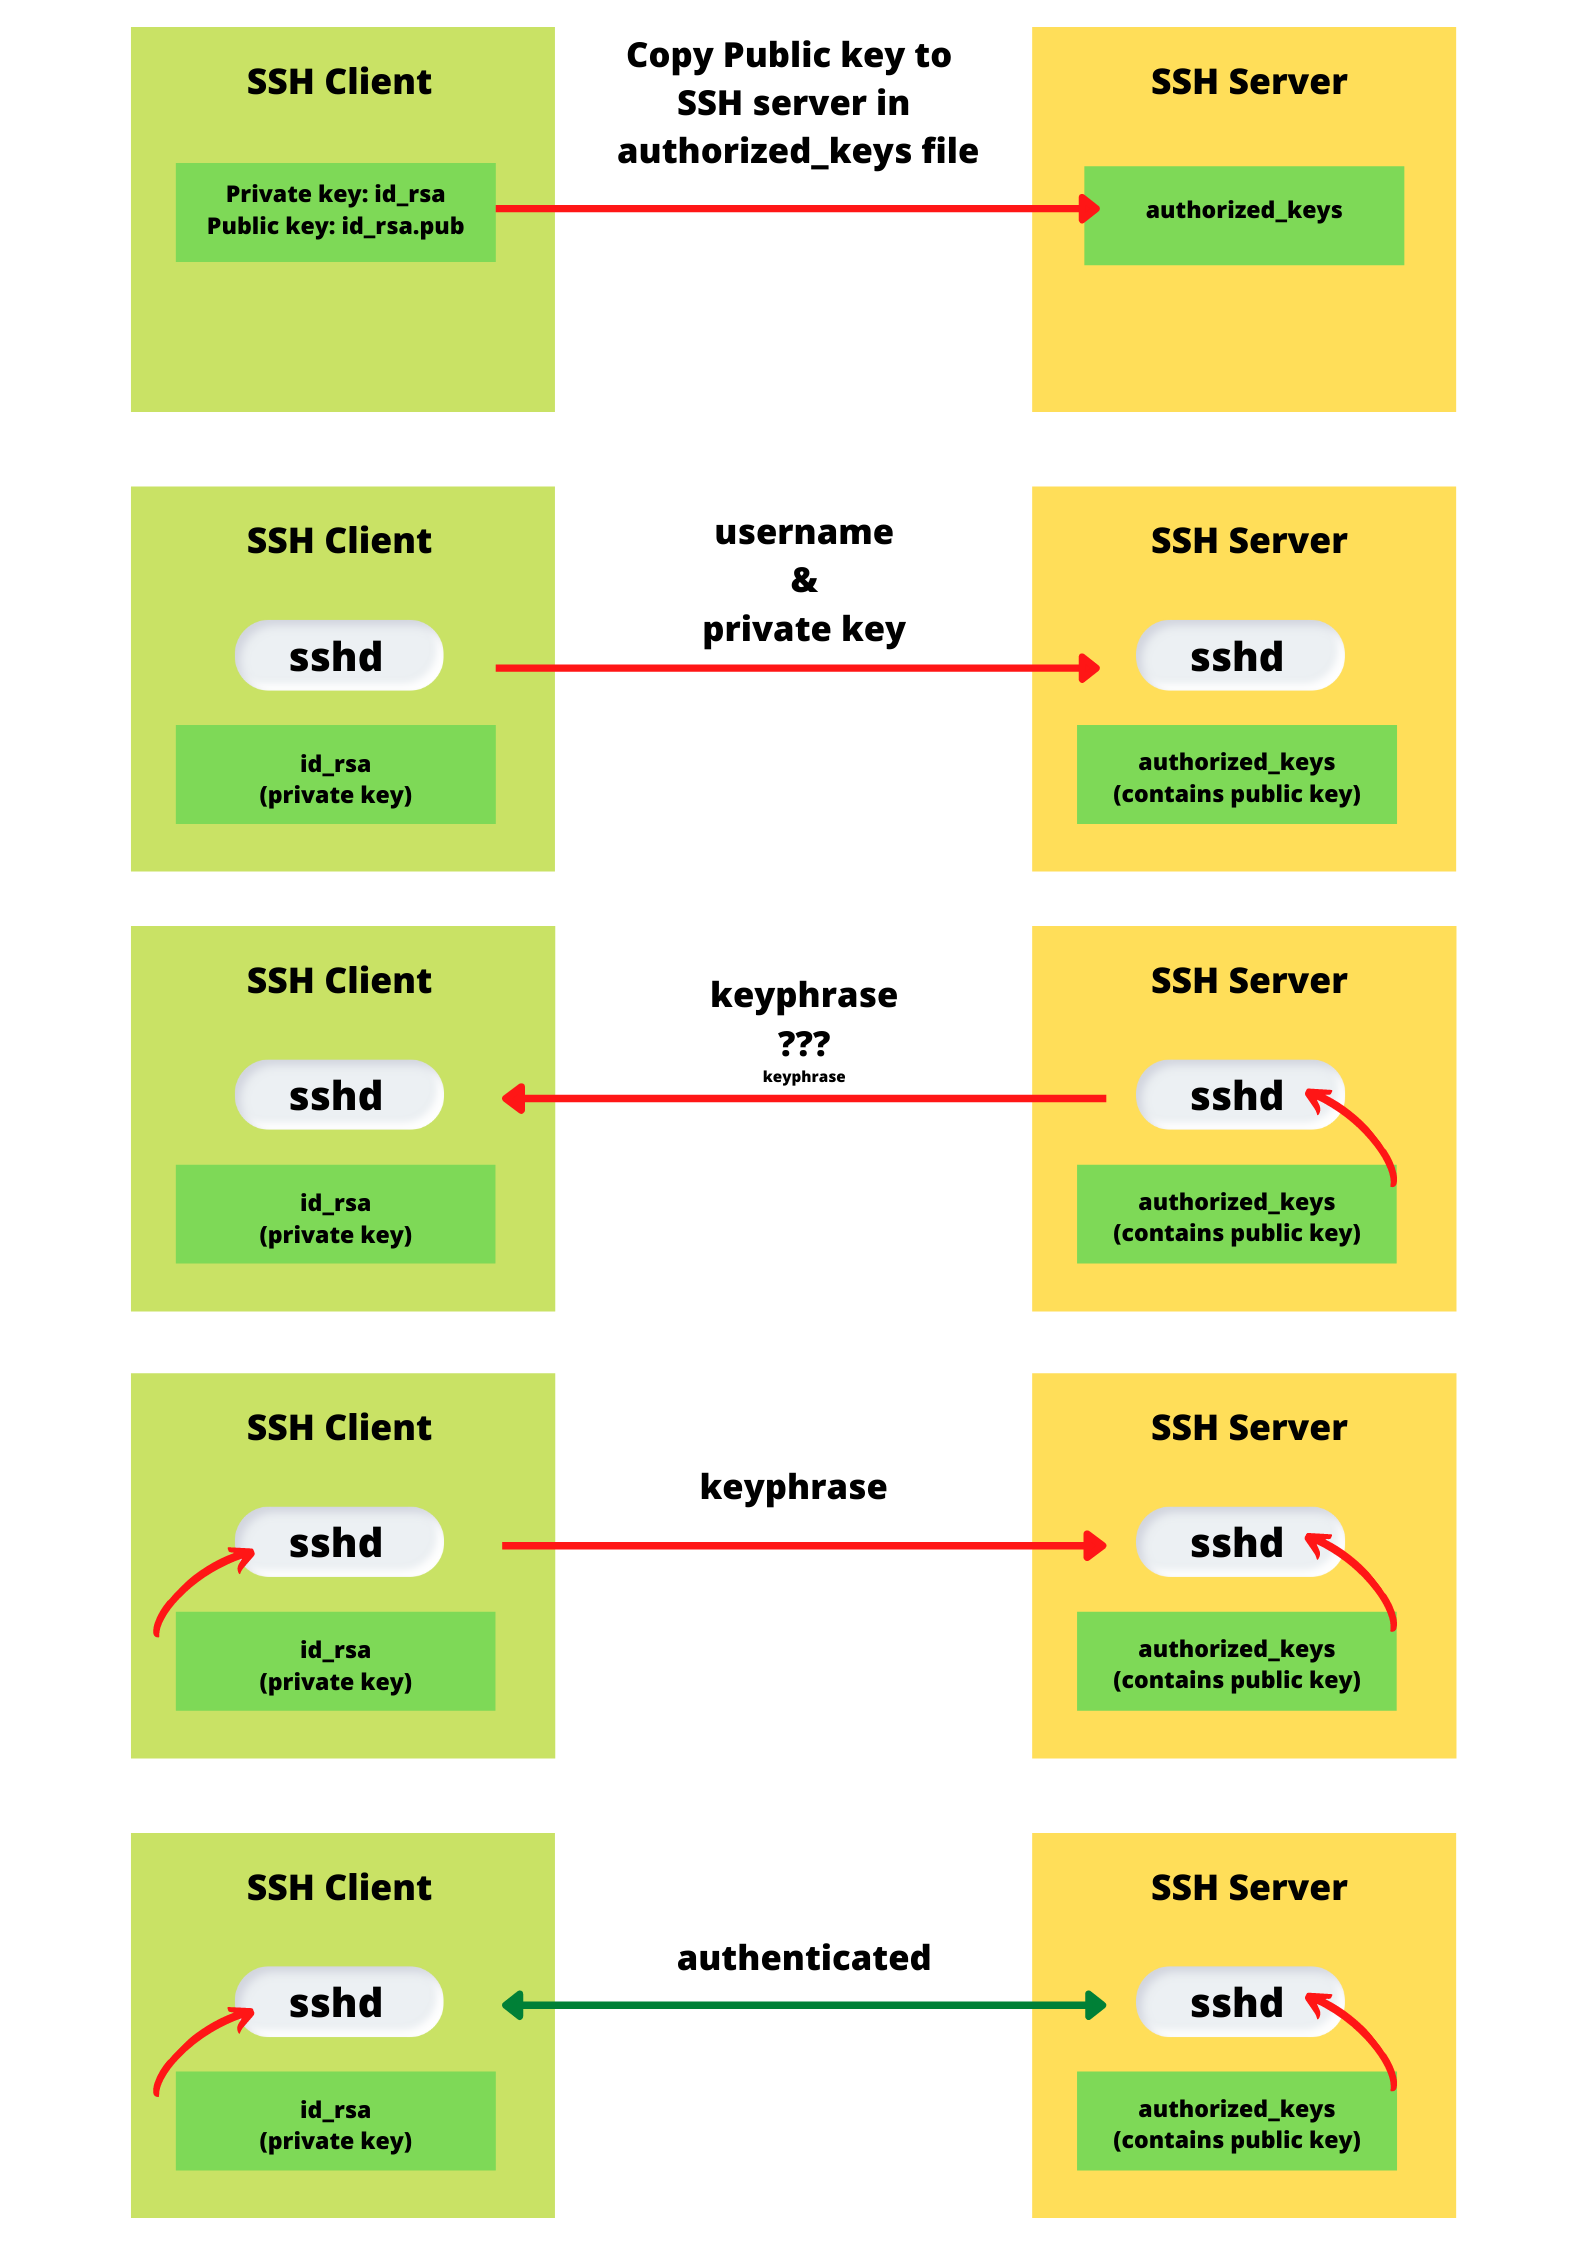
\includegraphics[scale=0.25]{content/chapter19/images/final.png}
		\caption{Working of Passwordless SSH}
		\label{fig:stage55635}
	\end{figure}
	
\end{itemize}

\newpage
\paragraph{Steps to configure Passwordless SSH}

\textbf{On SSH client:}
\begin{itemize}
	\item \textbf{Generate public-private key-pair}:
	\begin{itemize}
		\item \textbf{ssh-keygen}: Used to generate the key pair.
		\begin{tcolorbox}[breakable,notitle,boxrule=0pt,colback=pink,colframe=pink]
			\color{black}
			\fontdimen2\font=1em
			Syntax: ssh-keygen
			\fontdimen2\font=4pt
		\end{tcolorbox}
		
		\item Public key is generated as \textbf{$\sim$/.ssh/id\_rsa.pub} \& private key is generated as \textbf{$\sim$/.ssh/id\_rsa}.
		\item By default, RSA algorithm is used key-pair. Other algorithms are DSA, EDSA etc.
	\end{itemize}

	\begin{figure}[h!]
		\centering
		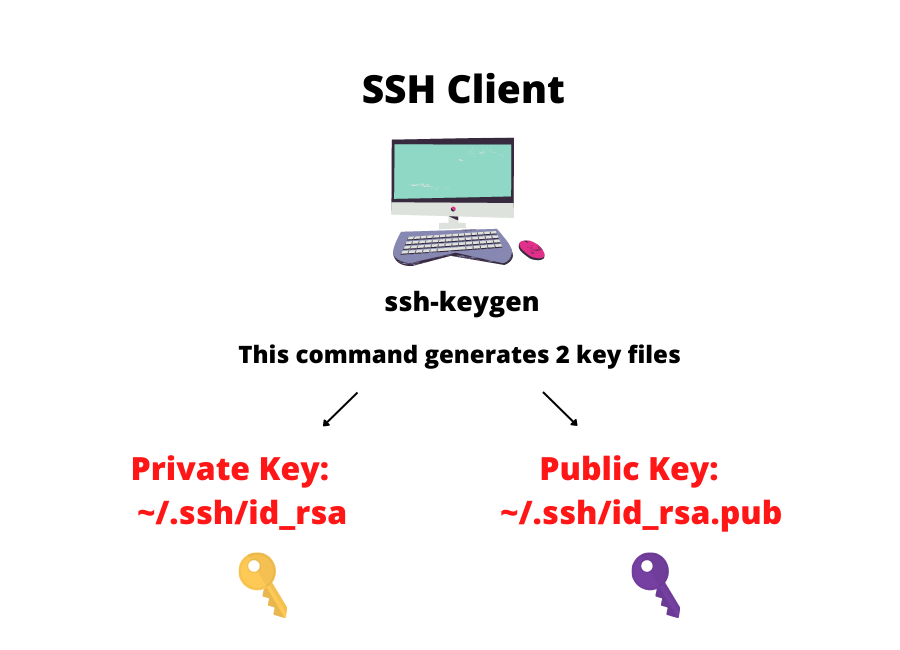
\includegraphics[scale=0.4]{content/chapter19/images/ssh0.png}
		\caption{Public \& Private key pair}
		\label{fig:stage5563}
	\end{figure}
	
	Eg:
	\begin{figure}[h!]
		\centering
		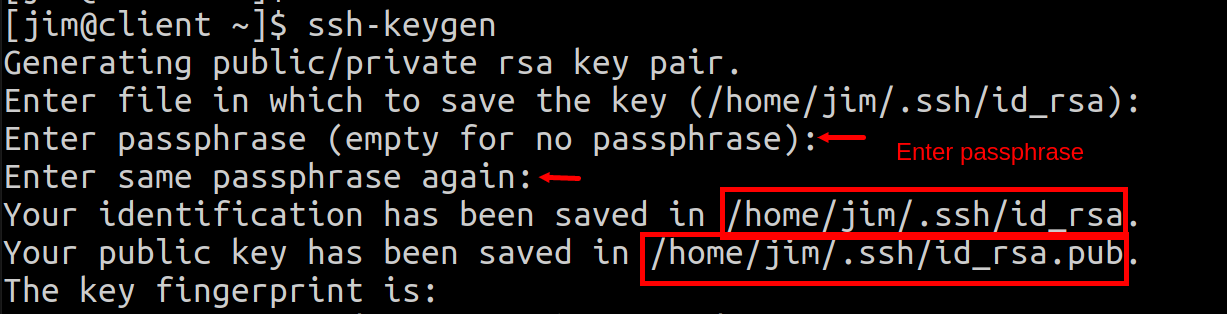
\includegraphics[scale=0.2]{content/chapter19/images/ssh9.png}
		\caption{Sample output}
		\label{fig:stage7}
	\end{figure}
	
		
	\newpage
	
	\item \textbf{Copy public-key from SSH client to SSH server:}
	\begin{itemize}
		\item \textbf{ssh-copy-id}: Copy public key (eg. $\sim$/.ssh/id\_rsa.pub) to SSH server in \textbf{$\sim$/.ssh/authorized\_keys} file.
		\item This command will ask you the \textbf{password of user's account on SSH server}.
		\bigskip
		\begin{tcolorbox}[breakable,notitle,boxrule=-0pt,colback=yellow,colframe=yellow]
			\color{black}
			Note: In order to copy keys, SSH server's \textbf{/etc/ssh/sshd\_config}  file should have setting:  \textbf{"PasswordAuthentication yes"}. 
		\end{tcolorbox}
		
		\bigskip
		\begin{tcolorbox}[breakable,notitle,boxrule=0pt,colback=pink,colframe=pink]
			\color{black}
			\fontdimen2\font=1em
			Syntax: ssh-copy-id  username@server\_ip\_address
			\fontdimen2\font=4pt
		\end{tcolorbox}
		
		\begin{figure}[h!]
			\centering
			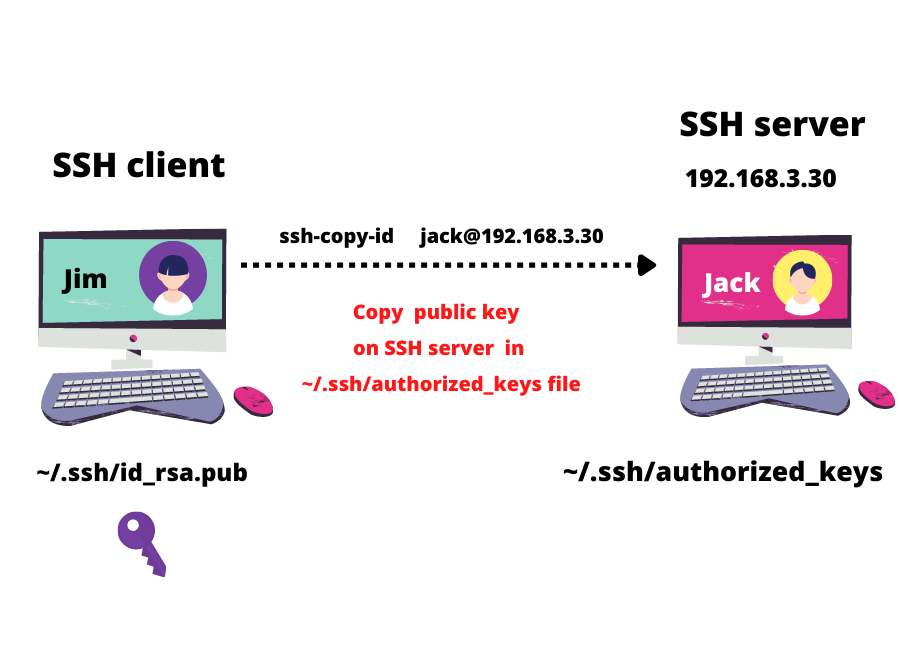
\includegraphics[scale=0.4]{content/chapter19/images/ssh01.png}
			\caption{Copy public key from SSH client to SSH server}
			\label{fig:stage556}
		\end{figure}
			
		Eg:
		\begin{figure}[h!]
			\centering
			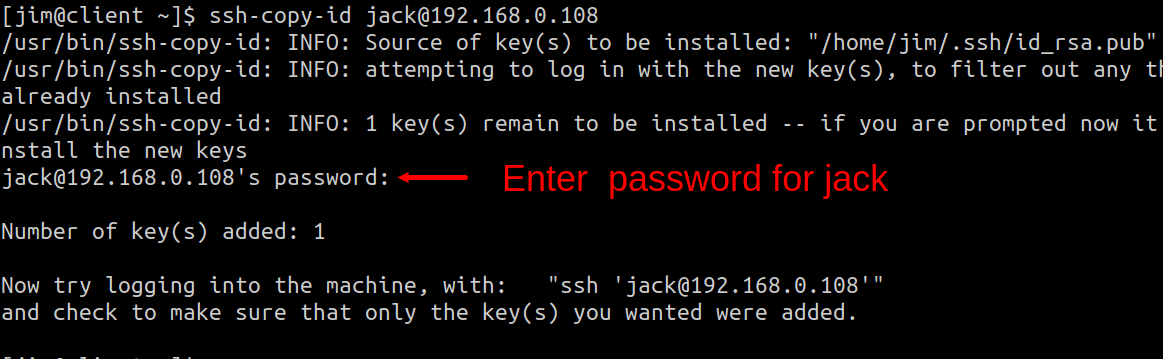
\includegraphics[scale=0.25]{content/chapter19/images/ssh09.png}
			\caption{Sample output}
			\label{fig:stage5569}
		\end{figure}

		\end{itemize}			
	\newpage
	
	\item \textbf{Finally from SSH client, take passwordless SSH of SSH server}:
		Eg:
	\begin{figure}[h!]
		\centering
		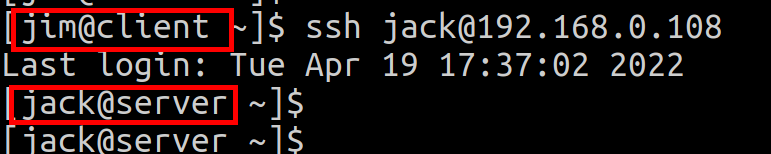
\includegraphics[scale=0.4]{content/chapter19/images/ssh07.png}
		\caption{Sample output}
		\label{fig:stage55693}
	\end{figure}
	
\end{itemize}		

\paragraph{On SSH server}

\begin{itemize}
	\item 	Once you have configured passwordless SSH, disable password based login permanently.
	
	\begin{tcolorbox}[breakable,notitle,boxrule=-0pt,colback=black,colframe=black]
		\color{green}
		\# grep  -w  PasswordAuthentication   /etc/ssh/sshd\_config 
		\newline
		\color{white}
		PasswordAuthentication no
		\fontdimen2\font=4pt
	\end{tcolorbox}
	\item 	Restart sshd daemon to reflect the changes in configuration file.
	
	\bigskip
	\begin{tcolorbox}[breakable,notitle,boxrule=-0pt,colback=black,colframe=black]
		\color{green}
		\fontdimen2\font=1em
		\# systemctl restart sshd
		\fontdimen2\font=4pt
	\end{tcolorbox}
	
\end{itemize}

	
	
	
	
	
	\newpage
	\paragraph{Important things to note about SSH server \& client}
	%\begin{tabulary}{1.0\textwidth}{C|C|C|p{10em}}
	
	
	\begin{tabulary}{1.0\textwidth}{|p{14em}|p{14em}|}
		\toprule
		SSH Port & 22 \\
		\hline
		SSH server package name & openssh-server \\
		\hline
		SSH client package name & openssh-client \\
		\hline
		Configuration file & /etc/ssh/sshd\_config \\
		\hline
		Daemon name & sshd \\
		\hline
		Location of public-private key-pair on SSH client & $\sim$/.ssh/ \\
		\hline
		Passwordless ssh command executed on SSH client & ssh-keygen, ssh-copy-id \\
		\hline
	\end{tabulary}
	
	\label{tab:example} % Unique label used for referencing the table in-text
	%\addcontentsline{toc}{table}{Table \ref{tab:example}} % Uncomment to add the table to the table of contents

	
	
	
	

	

	
	


\end{flushleft}
\newpage


